
\chapter{Systembeskrivelse}
Universal Actuator Drive består af to overordnede blokke. Et power-modul, der står for effektkonverteringen i converteren. Derudover et PWM-modul, der sikrer reguleringen af converterens udgang. Power-modulet består af en transformator og en MOSFET til convertering af udgangsbelastningen. Desuden et indgangs- og et udgangsfilter for filtrering af højfrekvent støj.

PWM-modulet består af to reguleringssløjfer, der regulerer udgangen efter både udgangsstrømmen og -spændingen. Denne regulering sker ved, at tilpasse duty-cyclen af det PWM-signal, der driver MOSFET'en. Disse funktionaliteter er inkluderet i PWM-controlleren. 

På figur~\ref{fig:flowdiagram} ses et flowdiagram for konceptet af Universal Actuator Drive. Det giver et overblik over hvilke scenarier, og eksterne valg, der kan påvirke flowet i systemet. Her er det især valg af udgangsbelastning, og de to reguleringssløjfer, der påvirker systemets udgang.

Systemet bliver initieret ved valg af udgangsbelastning. Det indstiller reguleringssløjferne, således at de regulerer efter den ønskede udgangsbelastning. Når belastningen aktiveres, begynder selve converterens funktionalitet. Den tilpasser switch-signalets duty-cycle efter både udgangsstrøm og -spænding, således den ønskede belastning holdes. Det forstætter indtil systemet deaktiveres, og indgangsspændingen til converteren fjernes. 

\begin{figure}[H]
	\centering
	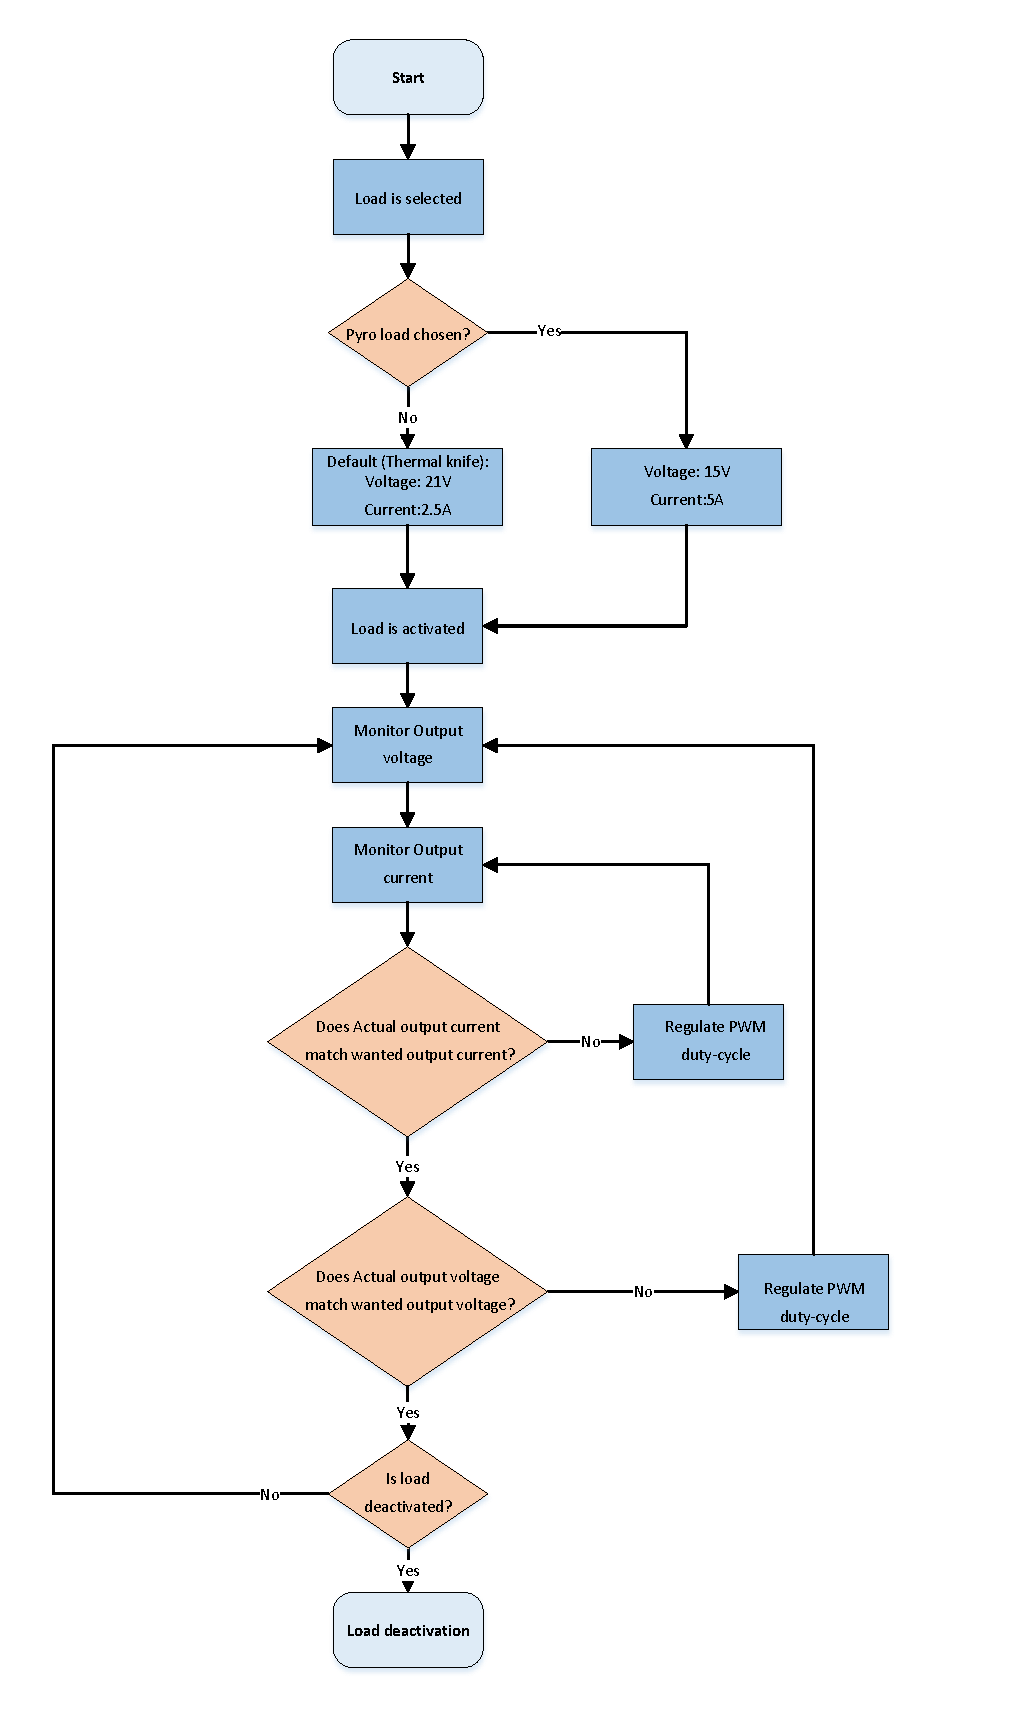
\includegraphics[width=0.7\linewidth]{../Dokumentation/tex/kravspecifikation/billeder/Flow_diagram.pdf}
	\caption{Flowdiagram for Universal Actuator Drive}
	\label{fig:flowdiagram}
\end{figure}